\documentclass[11pt,a4paper]{article}

\usepackage[T1]{fontenc}
\usepackage[utf8]{inputenc}
\usepackage{lmodern}
\usepackage[margin=2.5cm]{geometry}
\usepackage{amsmath}
\usepackage{amssymb}
\usepackage{booktabs}
\usepackage{graphicx}
\usepackage{caption}
\usepackage{listings}
\usepackage{xcolor}
\usepackage{microtype}
\usepackage[hidelinks]{hyperref}

\definecolor{linkblue}{HTML}{1C5CAB}
\definecolor{codebg}{HTML}{F5F5F3}
\definecolor{codegray}{HTML}{52514E}

\hypersetup{colorlinks=true, linkcolor=linkblue, urlcolor=linkblue, citecolor=linkblue}

\lstset{
  basicstyle=\ttfamily\footnotesize,
  backgroundcolor=\color{codebg},
  commentstyle=\color{codegray}\itshape,
  keywordstyle=\color{linkblue},
  breaklines=true,
  frame=none,
  xleftmargin=1em,
  framexleftmargin=1em,
  aboveskip=1em,
  belowskip=1em,
  showstringspaces=false,
  language=Python,
}

\captionsetup{font=small, labelfont=bf}

\title{\textbf{Predicting Interdimensional Transport on the Spaceship Titanic}\\[0.3em]
       \large A Feed-Forward Neural Network Implemented from First Principles}

\author{Ramez Ezzat\\
        \small Alamein International University\\
        \small \texttt{ramez.e.asaad@gmail.com}}

\date{\small Neural Networks (AIE231), Fall 2024/25 \\ \small Revised July 2026}

\begin{document}

\maketitle

\begin{abstract}
\noindent
This report describes a binary classifier for the Kaggle Spaceship Titanic
competition, which asks whether a given passenger was transported to an
alternate dimension during a collision with a spacetime anomaly. The classifier
is a fully connected neural network with three hidden layers, implemented
directly in NumPy: forward propagation, backpropagation, Xavier initialisation,
inverted dropout and mini-batch stochastic gradient descent are all written by
hand rather than delegated to an autograd framework. The gradients produced by
the hand-derived backward pass agree with central-difference numerical gradients
to a maximum relative error of $7.0\times10^{-8}$. On a stratified holdout the
model reaches 80.8\% accuracy, against a 77.8\% logistic regression floor and
79.7\% for an equivalent Keras model trained on identical features. The
discussion covers why the framework model does slightly worse, why the
validation loss sits below the training loss, and what the model's remaining
errors have in common.
\end{abstract}

\section{Problem}

The Spaceship Titanic dataset~\cite{kaggle} describes 12{,}970 passengers of a
fictional interstellar liner, roughly half of whom were transported to an
alternate dimension when the ship struck a spacetime anomaly. Each record holds
identifying information, cabin assignment, travel details and itemised billing
for five onboard amenities. The task is binary classification: predict the
boolean \texttt{Transported}.

The data splits into 8{,}693 labelled training rows and 4{,}277 unlabelled test
rows. The target is close to evenly balanced, at 50.4\% transported against
49.6\% not, so unweighted accuracy is a reasonable headline metric and a
majority-class baseline sits at 50.4\%.

Every feature column contains missing values, at a rate of roughly 2\% per
column. Imputation is therefore part of the problem rather than a preliminary to
it, and Section~\ref{sec:features} treats it as such.

\section{Data and features}
\label{sec:features}

\subsection{What predicts transport}

The dominant signal in the dataset is the interaction between cryosleep and
spending. Passengers who elected suspended animation are confined to their
cabins for the voyage, so they cannot use any amenity and their billing is
identically zero. This group is transported at a much higher rate than the
passengers who stayed awake. Spending, in other words, is not merely correlated
with the target: it is a near-deterministic proxy for a passenger's physical
state during the anomaly.

Two consequences follow, and both shape the pipeline. First, the five spending
columns and their aggregate carry more information than any demographic
variable. Second, a missing \texttt{CryoSleep} value is often recoverable: a
passenger billed for room service was demonstrably awake.

\subsection{Feature construction}

Thirteen raw columns are engineered into 33 model features.

\paragraph{Cabin.} The \texttt{Cabin} field has the form \texttt{deck/num/side}
and is split into its three parts. Deck and side are treated as categorical;
the cabin number is kept as a numeric feature.

\paragraph{Categorical encoding.} \texttt{HomePlanet}, \texttt{Destination},
\texttt{Cabin\_Deck} and \texttt{Cabin\_Side} are one-hot encoded, each with an
explicit \texttt{Unknown} level that absorbs missing values. One-hot encoding is
used deliberately in place of integer codes. Deck labels A through T have no
natural order, so mapping them to $0,\dots,7$ would assert both a ranking and a
uniform spacing between adjacent decks, neither of which exists in the domain. A
model given integer codes must then spend capacity undoing a false assumption
that the encoding introduced.

\paragraph{Group structure.} The \texttt{PassengerId} field has the form
\texttt{gggg\_pp}, where \texttt{gggg} identifies a travel group. Counting
members per group yields \texttt{GroupSize}, and \texttt{IsAlone} flags solo
travellers. Passengers travelling together share a fate more often than chance
would predict, so group size carries real signal that the raw ID hides.

\paragraph{Spending.} Amenity billing is heavily right-skewed: most passengers
spend nothing, and a thin tail spends thousands. Each spending column is
transformed with $\log(1+x)$, which compresses the tail onto a scale comparable
to the other standardised features while preserving order and keeping the exact
zeros at zero. A \texttt{TotalSpend} aggregate and a binary \texttt{NoSpend} flag
are added, the latter because ``spent nothing at all'' is a qualitatively
different state from ``spent very little'' and a linear feature cannot express
that distinction on its own.

Note that a naive outlier filter is counterproductive here. Discarding rows by a
$|z| > 3$ rule on skewed spending data removes precisely the high-spending
passengers whose records most sharply identify the awake population. The
$\log(1+x)$ transform addresses the scale problem without discarding anyone.

\paragraph{Imputation.} Missing spending is treated as a true zero: an unbilled
amenity is one the passenger did not use. Missing \texttt{CryoSleep} is inferred
from the resulting total, so that a passenger with any billing is marked awake
and one with none is assumed asleep. Remaining numeric gaps take the training
median, and categorical gaps take the explicit \texttt{Unknown} level rather than
a mode, since ``not recorded'' is itself informative given the ship's damaged
computer system.

All nine numeric features are standardised to zero mean and unit variance using
statistics computed on the training split only.

\section{Model}

\subsection{Architecture}

The classifier is a fully connected network with layer widths
$33 \rightarrow 128 \rightarrow 128 \rightarrow 128 \rightarrow 1$. Hidden layers
use ReLU, the output uses a sigmoid, and training minimises binary cross-entropy.
Dropout is applied after each hidden layer.

Writing $A^{[0]} = X$ for a batch of $m$ examples, the forward pass for each
layer $l$ is

\begin{equation}
Z^{[l]} = A^{[l-1]} W^{[l]} + b^{[l]},
\qquad
A^{[l]} =
\begin{cases}
\mathrm{ReLU}\!\left(Z^{[l]}\right) \odot M^{[l]} & l < L,\\[0.35em]
\sigma\!\left(Z^{[l]}\right) & l = L,
\end{cases}
\end{equation}

where $W^{[l]} \in \mathbb{R}^{n_{l-1} \times n_l}$, $b^{[l]} \in
\mathbb{R}^{1 \times n_l}$, and $M^{[l]}$ is the dropout mask of
Section~\ref{sec:dropout}. The loss over the batch is

\begin{equation}
\mathcal{L} = -\frac{1}{m}\sum_{i=1}^{m}
\left[ y_i \log \hat{y}_i + (1-y_i)\log(1-\hat{y}_i) \right].
\end{equation}

\subsection{Numerically stable sigmoid}

Evaluating $\sigma(z) = 1/(1+e^{-z})$ directly overflows for large negative $z$,
since $e^{-z}$ grows without bound. The implementation branches on sign and uses
the algebraically equivalent form for the negative case:

\begin{equation}
\sigma(z) =
\begin{cases}
\dfrac{1}{1+e^{-z}} & z \geq 0,\\[0.9em]
\dfrac{e^{z}}{1+e^{z}} & z < 0.
\end{cases}
\end{equation}

Each branch only ever exponentiates a non-positive number, so the argument to
$\exp$ is bounded above by zero and the result is finite for every input. The
test suite checks this at $z = \pm 1000$.

\subsection{Weight initialisation}

Weights use Xavier (Glorot) uniform initialisation~\cite{glorot}, drawing from

\begin{equation}
W^{[l]} \sim \mathcal{U}\!\left[
-\sqrt{\frac{6}{n_{l-1}+n_l}},\;
\sqrt{\frac{6}{n_{l-1}+n_l}}
\right],
\end{equation}

with biases initialised to zero. The bound keeps the variance of activations and
gradients roughly constant across layers, which matters at depth: initialise too
small and the signal vanishes as it propagates, too large and it saturates.

Xavier is derived under an assumption of a symmetric activation with unit
derivative at the origin, which fits the sigmoid output better than the ReLU
hidden layers. He initialisation~\cite{he}, which scales by $\sqrt{2/n_{l-1}}$,
is the more principled choice for ReLU because it accounts for the expected
halving of variance when negative pre-activations are zeroed. Xavier is retained
here for consistency with the original specification of the project, and at this
depth the practical difference is small.

\subsection{Dropout}
\label{sec:dropout}

Training applies inverted dropout to each hidden layer. With keep probability
$p = 1 - r$ for dropout rate $r$, the mask is

\begin{equation}
M^{[l]}_{ij} = \frac{1}{p}\,\mathbb{1}\!\left[u_{ij} < p\right],
\qquad u_{ij} \sim \mathcal{U}[0,1].
\end{equation}

Scaling by $1/p$ at training time preserves the expected value of each
activation, $\mathbb{E}[a \odot M] = a$, which means inference can use the
network unmodified with no compensating rescale. The alternative, scaling at test
time, moves the correction to the hot path and is easier to get wrong.

\subsection{Backpropagation}

The output layer gradient is where the choice of loss pays off. For a sigmoid
output under binary cross-entropy, the derivative of the loss with respect to the
pre-activation simplifies. Writing $\hat{y} = \sigma(z)$ and using
$\sigma'(z) = \sigma(z)(1-\sigma(z))$:

\begin{align}
\frac{\partial \mathcal{L}}{\partial \hat{y}}
  &= \frac{1}{m}\left(\frac{1-y}{1-\hat{y}} - \frac{y}{\hat{y}}\right)
   = \frac{1}{m}\cdot\frac{\hat{y}-y}{\hat{y}(1-\hat{y})},\\[0.5em]
\frac{\partial \mathcal{L}}{\partial z}
  &= \frac{\partial \mathcal{L}}{\partial \hat{y}} \cdot \sigma'(z)
   = \frac{1}{m}\cdot\frac{\hat{y}-y}{\hat{y}(1-\hat{y})} \cdot \hat{y}(1-\hat{y})
   = \frac{\hat{y}-y}{m}.
\end{align}

The $\hat{y}(1-\hat{y})$ factor cancels exactly. This is not a convenience: it is
the reason sigmoid pairs with cross-entropy rather than with squared error. Under
squared error the factor survives, and it approaches zero whenever the sigmoid
saturates, so a confidently wrong prediction would receive almost no gradient and
the network would learn most slowly precisely where it is most wrong.

With $\mathrm{d}Z^{[L]} = (A^{[L]} - y)/m$ established, gradients flow back
through each layer as

\begin{align}
\mathrm{d}W^{[l]} &= \left(A^{[l-1]}\right)^{\!\top} \mathrm{d}Z^{[l]},\\
\mathrm{d}b^{[l]} &= \sum_{i=1}^{m} \mathrm{d}Z^{[l]}_{i},\\
\mathrm{d}Z^{[l-1]} &= \left(\mathrm{d}Z^{[l]} \left(W^{[l]}\right)^{\!\top}
  \odot M^{[l-1]}\right) \odot \mathbb{1}\!\left[Z^{[l-1]} > 0\right].
\end{align}

The dropout mask reappears in the backward pass because the same units that were
zeroed on the way forward must not receive gradient on the way back. Parameters
then update by plain stochastic gradient descent,
$W^{[l]} \leftarrow W^{[l]} - \eta\,\mathrm{d}W^{[l]}$, over shuffled mini-batches
of 32.

\subsection{Gradient verification}

A hand-derived backward pass is worth only as much as its correctness, and a
network with a subtly wrong gradient will often still train, just worse. The
implementation is therefore checked against central differences,

\begin{equation}
\frac{\partial \mathcal{L}}{\partial W_{ij}} \approx
\frac{\mathcal{L}(W_{ij}+\epsilon) - \mathcal{L}(W_{ij}-\epsilon)}{2\epsilon},
\qquad \epsilon = 10^{-6},
\end{equation}

with the relative error measured as

\begin{equation}
\text{error} = \frac{\left|\nabla_{\text{numerical}} - \nabla_{\text{analytic}}\right|}
{\left|\nabla_{\text{numerical}}\right| + \left|\nabla_{\text{analytic}}\right|}.
\end{equation}

Dropout is disabled for the check, since a stochastic loss makes the two
evaluations of $\mathcal{L}$ incomparable. Across all layers the maximum relative
error is $6.96\times10^{-8}$, consistent with floating-point noise rather than a
derivation error. The check runs in the test suite on every commit.

\section{Experiments}

\subsection{Setup}

All models are evaluated on a stratified 20\% holdout of the training data
(6{,}954 train, 1{,}739 validation) with seed 42. The network trains for 60
epochs at a learning rate of 0.01, batch size 32, dropout 0.2.

The learning rate was selected by sweep. At $\eta = 0.001$ plain SGD has not
converged within the epoch budget, reaching only 78.9\% after 150 epochs. At
$\eta = 0.05$ the model overfits, separating to 88.9\% train against 79.9\%
validation. The chosen value of 0.01 sits at the optimum of the sweep.

\subsection{Results}

\begin{table}[h]
\centering
\caption{Validation performance. Feature counts differ because the 2024
pipeline row uses the original six-column feature set.}
\vspace{0.4em}
\begin{tabular}{lcccc}
\toprule
\textbf{Model} & \textbf{Features} & \textbf{Accuracy} & \textbf{F1} & \textbf{ROC AUC} \\
\midrule
Majority class          & n/a & 50.4\% & n/a   & n/a   \\
2024 pipeline           & 6  & 73.4\% & 0.707 & 0.791 \\
Logistic regression     & 33 & 77.8\% & 0.781 & 0.860 \\
Keras equivalent (Adam) & 33 & 79.7\% & 0.800 & 0.886 \\
\textbf{From-scratch network} & 33 & \textbf{80.8\%} & \textbf{0.804} & \textbf{0.896} \\
\bottomrule
\end{tabular}
\label{tab:results}
\end{table}

\begin{figure}[h]
\centering
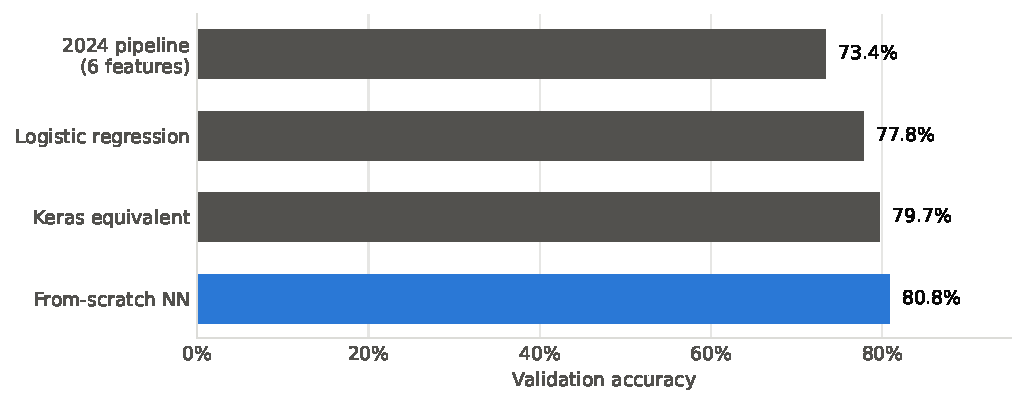
\includegraphics[width=\textwidth]{figures/model-comparison.pdf}
\caption{Validation accuracy by model. The logistic regression bar is the
relevant floor: it is what the network must beat to justify its own complexity.}
\end{figure}

The logistic regression row is the control that gives the headline number
meaning. A network reaching 80.8\% is only interesting relative to what a linear
model extracts from the same features, and the three-point margin is what
establishes that the interactions in this dataset are genuinely non-linear. The
largest of those interactions is cryosleep against spending, which a linear model
in these features cannot represent: the effect of spending on transport
probability depends on a passenger's cryosleep state rather than adding to it.

\subsection{Training behaviour}

\begin{figure}[h]
\centering
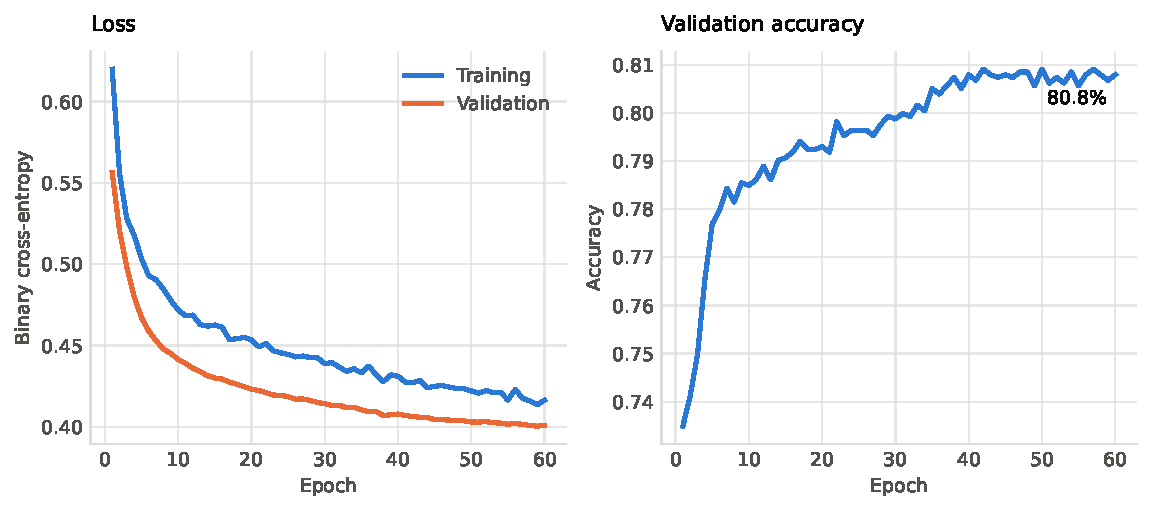
\includegraphics[width=\textwidth]{figures/training-curves.pdf}
\caption{Training dynamics over 60 epochs. Validation loss falls below training
loss throughout, which is a consequence of dropout rather than a defect.}
\label{fig:curves}
\end{figure}

Figure~\ref{fig:curves} shows validation loss sitting consistently below training
loss, which inverts the usual relationship and is worth explaining. Training loss
is measured with dropout active, so roughly a fifth of each hidden layer is
zeroed while the loss is computed. Validation runs the full network. The
training figure is therefore the loss of a deliberately handicapped model, and
the gap measures the handicap rather than any generalisation failure. The two
curves descend together and neither turns upward, which is the actual evidence
that the model is not overfitting.

\subsection{Why the framework model does worse}

The Keras model in Table~\ref{tab:results} uses the same architecture and the
same 33 features, differing only in optimiser: Adam rather than plain SGD. It
reaches 86.1\% training accuracy against 79.7\% validation, while the
from-scratch network reaches 80.8\% on both.

Adam's per-parameter adaptive learning rates let it descend the training
objective considerably faster, and on a dataset of this size that is not an
advantage. It fits the training split more tightly and generalises slightly
worse. The result is a reminder that the more sophisticated optimiser is not
automatically the better one, and that the metric worth watching is the one on
data the model has not seen.

\subsection{Error analysis}

The residual errors are concentrated, not diffuse. Passengers with no recorded
spending and no recorded cryosleep status are the single hardest group: the
inference rule of Section~\ref{sec:features} assigns them to cryosleep, which is
right more often than not but is a guess. Passengers who spent small amounts are
also disproportionately misclassified, sitting near the boundary the model has
learned between the awake and asleep populations.

This suggests the ceiling here is partly irreducible. A passenger who was awake
but simply bought nothing is, in these features, indistinguishable from one in
cryosleep. Published solutions to this competition cluster around 80\% to 81\%,
which is consistent with that reading.

\section{Deployment}

The trained model serialises to a 280\,KB compressed \texttt{.npz} holding the
weight and bias matrices. Inference is one matrix multiply per layer, so the
serving path depends on NumPy alone and no deep learning framework is installed
at runtime.

The preprocessing statistics serialise to plain JSON rather than a pickle. Every
value learned from the training data, the medians, means and standard deviations,
is stored as a number, so the transform can be reconstructed without
scikit-learn and there is no version-coupled binary artefact to break on a
library upgrade.

An interactive demonstration built with Streamlit accepts a passenger record and
returns a transport probability, together with a per-prediction sensitivity
analysis: each field is reset to a neutral value in turn and the resulting shift
in probability is reported. This is a local occlusion measure and not a global
feature importance, but it makes the cryosleep effect directly visible. Toggling
cryosleep on an otherwise fixed passenger moves the predicted probability by
roughly 0.20.

Model behaviour on hand-constructed records matches the domain: a passenger in
cryosleep with no billing scores 0.86, an awake passenger billed 2{,}900 across
amenities scores 0.09, and a record with every field unknown scores 0.40, close
to the base rate and appropriately uncertain.

\section{Conclusion}

A three-hidden-layer network written directly in NumPy reaches 80.8\% validation
accuracy on the Spaceship Titanic task, three points above a logistic regression
floor on identical features and one point above an equivalent Keras model. The
hand-derived backward pass is verified against numerical gradients to
$7.0\times10^{-8}$.

The result rests more on the feature work than on the architecture. Recognising
that cryosleep and amenity spending are two views of the same latent variable,
that a passenger's billing record reveals whether they were conscious, is what
moves the number. The choice to encode cabin decks without imposing a false
order, and to compress skewed spending with $\log(1+x)$ rather than discard the
tail as outliers, follow from taking the domain seriously rather than from
tuning.

Further gains would most likely come from the group structure. Passengers
travelling together share outcomes, and the current model sees only group size
rather than the fate of a passenger's companions.

\begin{thebibliography}{9}

\bibitem{kaggle}
Kaggle. \emph{Spaceship Titanic: Predict which passengers are transported to an
alternate dimension}. \url{https://www.kaggle.com/competitions/spaceship-titanic}

\bibitem{glorot}
X. Glorot and Y. Bengio. \emph{Understanding the difficulty of training deep
feedforward neural networks}. AISTATS, 2010.

\bibitem{he}
K. He, X. Zhang, S. Ren and J. Sun. \emph{Delving deep into rectifiers:
Surpassing human-level performance on ImageNet classification}. ICCV, 2015.

\bibitem{srivastava}
N. Srivastava, G. Hinton, A. Krizhevsky, I. Sutskever and R. Salakhutdinov.
\emph{Dropout: A simple way to prevent neural networks from overfitting}. JMLR,
15(56):1929-1958, 2014.

\end{thebibliography}

\vspace{1em}
\noindent\rule{\textwidth}{0.4pt}\\
\small
Source code, tests and the interactive demonstration are available at
\url{https://github.com/Ramez-Asaad/spaceship-titanic-neural-network}.

\end{document}
